\documentclass[]{article}
\usepackage[utf8]{inputenc}
\usepackage{polski}
\usepackage{graphicx}
\graphicspath{ {./images/} }
\usepackage[margin=0.5in]{geometry}
\usepackage{gensymb}
\usepackage{textcomp}
\usepackage{siunitx}
\usepackage{float}
\documentclass{article}
\usepackage{graphicx}
\usepackage{wrapfig}
\usepackage{lipsum}
\usepackage{graphicx}
\usepackage{subcaption}
\begin{document}

\begin{figure}[tp!]
	\center{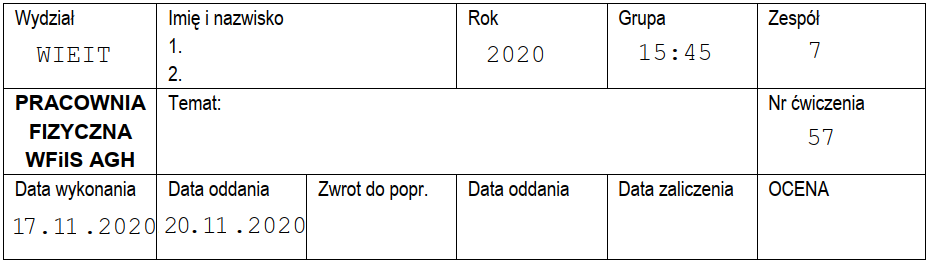
\includegraphics{F}}
\end{figure}

\begin{center}
	\section*{Współczynnik załamania światła dla ciał stałych }
	\emph{Dzmitry Mikialevich}
\end{center}
\begin{center}
	\emph{Wojciech Sikora}
\end{center}
\tableofcontents
\newpage

\section{Wstęp}

\subsection{Cel ćwiczenia}
Wyznaczenie współczynnika załamania światła dla wody oraz oleju.

    


    
\section{Układ Pomiarowy}
W skład układu pomiarowego weszły następujące elementy:
\newline

1. Szklanka o cienkich ściankach


2. Pasek papieru lekko prześwitującego z wyciętą wąską szczeliną i plaster


3. Latarka z komórki jako źródło światła

4.Linijka

5.Książki jako podstawka pod źródło światła

6.Woda, olej (rzepakowy)

\begin{figure}[H]
  \centering
  \begin{subfigure}[b]{0.4\linewidth}
    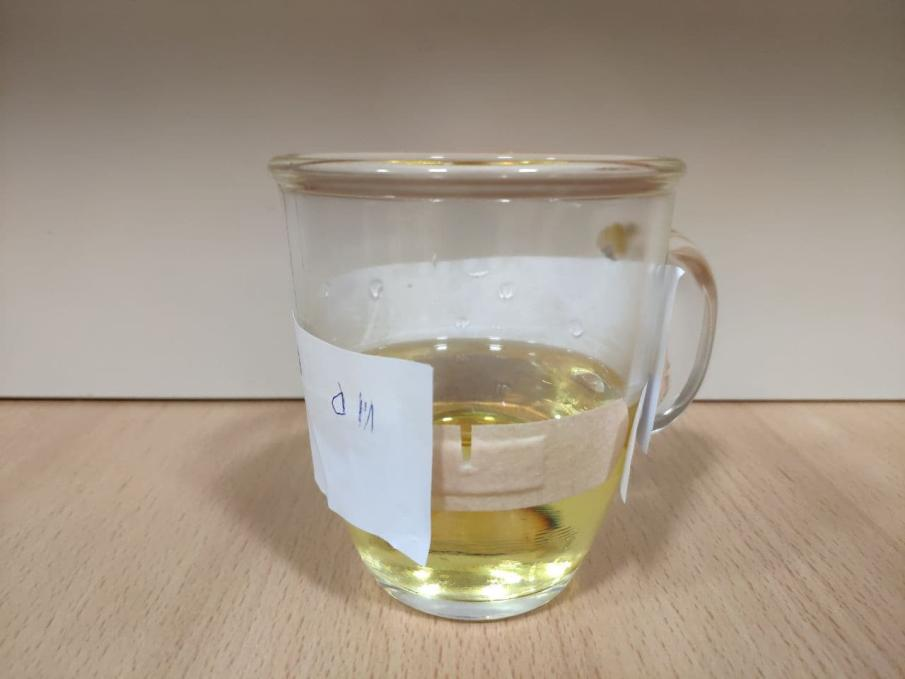
\includegraphics[width=\linewidth]{1}
    \caption{Szklanka z olejem}
  \end{subfigure}
  \begin{subfigure}[b]{0.4\linewidth}
    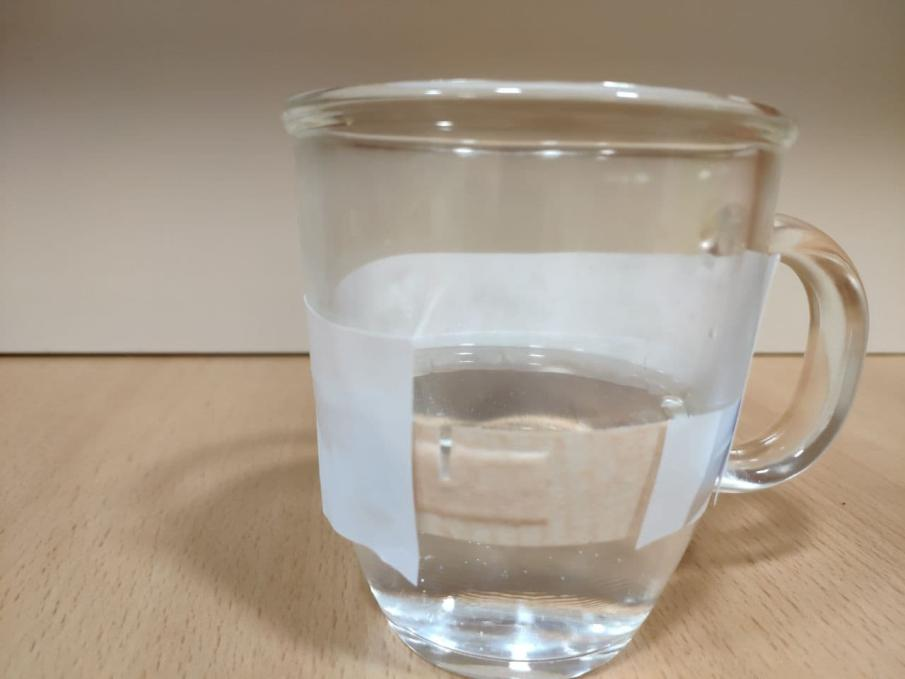
\includegraphics[width=\linewidth]{2}
    \caption{Szklanka z wodą}
  \end{subfigure}
  \begin{subfigure}[b]{0.4\linewidth}
    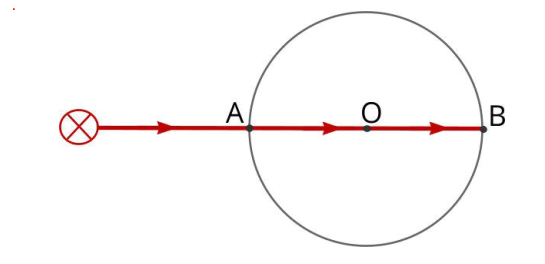
\includegraphics[width=\linewidth]{3}
    \caption{Promień światła biegnący
poniżej powierzchni cieczy }
  \end{subfigure}
  \begin{subfigure}[b]{0.4\linewidth}
    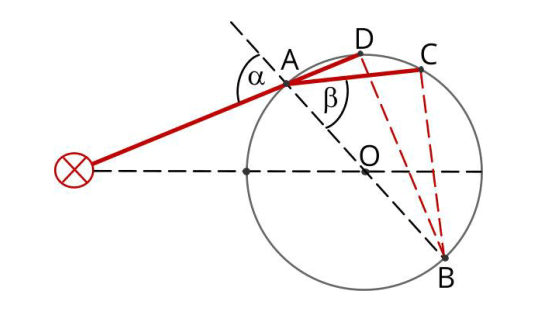
\includegraphics[width=\linewidth]{4}
    \caption{Bieg promienia przez powietrze}
  \end{subfigure}
  
\end{figure}




\section{Przebieg doświadczenia}
Na szklankę nakleiliśmy pasek prześwitującego papieru oraz kawałek plastra z wąską szczeliną. Następnie nalaliśmy do połowy naczynia najpierw wodę a potem olej.  Ustawiliśmy naczynie tak, aby źródło światła (latarka z komórki) leżała na jednej prostej wraz ze środkiem i szczeliną. Następnie obracaliśmy szklankę o pewien kąt i mierzyliśmy BD i BC (jak na rysunku powyżej) dla obu przypadków. 

\newpage

\section{Wyniki Pomiarów}

Obwód szklanki:
    \[l = 26,7\:cm\]
    \[u(l) = 1\:mm\]

Dla wody:

	\begin{table}[H]
		\centering
		\begin{tabular}{|l|l|l|l|}
			\hline
Numer Pomiaru & BD [cm]
& BC [cm] & \(n_w\) \\ \hline
1 & 8,1 & 6,1 & 1,3279 \\ \hline
2 & 7,9 & 6,0 & 1,3167 \\ \hline
3 & 7,6 & 5,6 & 1,3571 \\ \hline
4 & 7,0 & 5,3 & 1,3208 \\ \hline
5 & 6,2 & 4,6 & 1,3478 \\ \hline
6 & 5,9 & 4,5 & 1,3111 \\ \hline
7 & 5,8 & 4,3 & 1,3488 \\ \hline


		\end{tabular}
		\textbf{\caption{Wartość współczynnika załamania dla wody}
		}
	\end{table}

Dla oleju:	
		\begin{table}[H]
		\centering
		\begin{tabular}{|l|l|l|l|}
			\hline
Numer Pomiaru & BD [cm]& BC [cm]& \(n_{ol}\) \\ \hline
1 & 8,2 & 5,7 & 1,439 \\ \hline
2 & 7,9 & 5,4 & 1,463 \\ \hline
3 & 6,8 & 4,8 & 1,417 \\ \hline
4 & 6,3 & 4,5 & 1,400 \\ \hline
5 & 5,9 & 3,9 & 1,513 \\ \hline
6 & 5,7 & 3,8 & 1,500 \\ \hline
7 & 5,1 & 3,5 & 1,457 \\ \hline

		\end{tabular}
		\textbf{\caption{Wartość współczynnika załamania dla oleju}
		}
	\end{table}
	
	
\newline


\section{Opracowanie wyników Pomiarów}
    \subsection{Stosowany wzór}

\[n = \frac{BD}{BC}\]
    \subsection{Wartość średnia współczynnika załamania}
Wartość średnia wpółczynnika załamania dla wody:
    \[\overline n_w =1,3328 \]
Wartość średnia wpółczynnika załamania dla oleju:
    \[\overline n_{ol} = 1,455\]
\subsection{Niepewność typu B i typu A}
Niepewności typu B:
\[u(l) = 1\:mm\]
Niepewności typu A:
\[u(n_{w}) = \sqrt{\frac{\sum (n_{w_i} - \overline n_{w})^2}{n(n-1)}} = 0,00685565 \approx 0,0068\]
\[u(n_{ol}) = \sqrt{\frac{\sum (n_{ol_i} - \overline n_{ol})^2}{n(n-1)}} = 0,01558256 \approx 0,015\]

\subsection{Dopasowanie prostych}
	Parametry prostych były wygenerowane za pomocą funkcji LINEST w Excelu.
\begin{figure}[H]
	\center{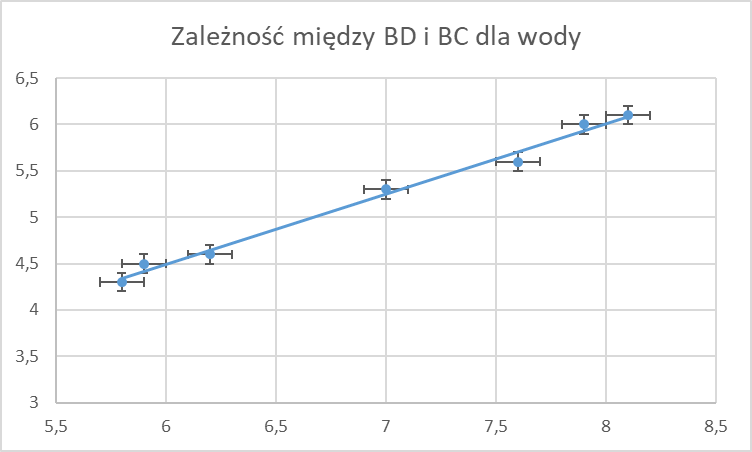
\includegraphics{w1}}
	\textbf{\caption{Wykres otrzymanych wartości wydłużenia drutu w funkcji  działającej siły zewnętrznej}}
\end{figure}

	
\begin{figure}[H]
	\center{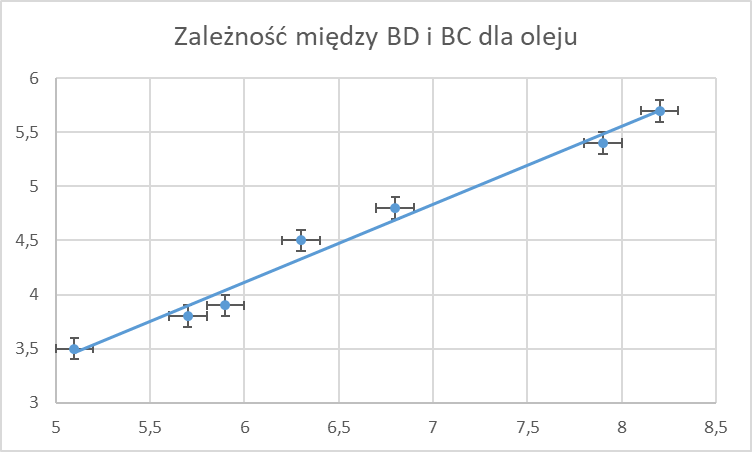
\includegraphics{w2}}
	\textbf{\caption{Wykres otrzymanych wartości wydłużenia drutu w funkcji  działającej siły zewnętrznej}}
\end{figure}



	\begin{table}[H]
		\centering
		\begin{tabular}{|l|l|l|l|l|l|l|}
			\hline
Płyn & 
\begin{tabular}{@{}c@{}}Wartość współczynnika\\ a \:  \end{tabular}
 & u(a) & \begin{tabular}{@{}c@{}}Wartość współczynnika\\ b \:  \end{tabular}& u(b)& \begin{tabular}{@{}c@{}}Wartość współczynnika\\korelacji y \:  \end{tabular} & u(y)  \\ \hline
Woda & 0,759634888 & 0,031952896 & -0,063184584 & 0,223236202 & 0,991230891 & 0,075845471 \\ \hline
Olej & 0,720498015 & 0,0445724 & -0,210122699 &0,296086718 & 0,981223934 & 0,125415225 \\ \hline

		\end{tabular}
		\textbf{\caption{Parametry prostych}
		}
	\end{table}


\subsection{Zestawienie wyników}
	\begin{table}[H]
		\centering
		\begin{tabular}{|l|l|l|l|l|}
			\hline
                Rodzaj płynu & Wartość n  & Niepewność u(n) & Tablicowe n  & Różnica \(\Delta n\)\\ \hline
                Woda & 1,3328 & 0,0068 & 1,33 & 0,0028 \\ \hline
                Olej & 1,455  & 0,015 & 1,47 &  0,015\\ \hline
		    
		\end{tabular}
		\textbf{\caption{Zestawienie wyników}
		}
	\end{table}
\subsection{Wnioski}
\begin{itemize}
		\item W przeprowadzonym doświadczeniu otrzymaliśmy wartości współczynnika załamania dla wody oraz oleju. 
		\newline
        \(n_w = 1,3328 \pm 0,0136\)\newline
        \(n_{ol} = 1,455 \pm 0,030\)
		\item Różnice wartości tablicowej współczynnika załamania światła, dla wody i dla oleju, i otrzymanych wartości  mieszczą się w granicach niepewnści rozszerzonej (a nawet standardowej).
		\item Widać, że punkty, w granicach niepewności rozszerzonej (a nawet standardowej co widać na wykresach) leżą na jednej prostej, co jeszcze raz podtwierdzają współczynniki korelacji bliskie do 1.
% 		\newline Średnia wartość współczynnika załamania dla wody \(\overline n_{w}=1,3328\). Średnia wartość współczynnika załamania dla oleju \(\overline n_{ol}=1,455\)
		
	\end{itemize}
\end{document}